\documentclass[12pt,a4paper,austrian]{article}
\usepackage{graphicx}
\usepackage[austrian, english]{babel}
\usepackage[utf8]{inputenc}
%\usepackage{listings}
\usepackage{multirow}
\usepackage{epstopdf}
\usepackage{amsmath}
\usepackage{amssymb} % fuer Mengen \N, Q, C, R
\usepackage{matlab-prettifier}
\graphicspath{{./fig/}}

\usepackage[colorlinks=true, pdfborder={0 0 0}, linkcolor=red]{hyperref}
\usepackage{float}


%% Satzspiegel
\setlength{\hoffset}{-1in} \setlength{\textwidth}{18cm}
\setlength{\oddsidemargin}{1.5cm}
\setlength{\evensidemargin}{1.5cm}
\setlength{\marginparsep}{0.7em}
\setlength{\marginparwidth}{0.5cm}

\setlength{\voffset}{-1.9in}
\setlength{\headheight}{12pt}
\setlength{\topmargin}{2.6cm}
   \addtolength{\topmargin}{-\headheight}
\setlength{\headsep}{3.5cm}
   \addtolength{\headsep}{-\topmargin}
   \addtolength{\headsep}{-\headheight}
\setlength{\textheight}{27cm}

%% How should floats be treated?
\setlength{\floatsep}{12 pt plus 0 pt minus 8 pt}
\setlength{\textfloatsep}{12 pt plus 0pt minus 8 pt}
\setlength{\intextsep}{12 pt plus 0pt minus 8 pt}

\tolerance2000
\emergencystretch20pt

%% Text appearence
% English text
\newcommand{\eg}[1]%
  {\selectlanguage{english}\textit{#1}\selectlanguage{austrian}}

\newcommand{\filename}[1]
  {\begin{small}\texttt{#1}\end{small}}

\newcommand\IFT{\unitlength1mm\begin{picture}(10,2) \put (1,1)
{\circle{1.7}} \put(2,1){\line(1,0){5}} \put(8,1)
{\circle*{1.7}}\end{picture}}
\newcommand\FT{\unitlength1mm\begin{picture}(10,2) \put (1,1)
{\circle*{1.7}} \put(2,1){\line(1,0){5}} \put(8,1)
{\circle{1.7}}\end{picture}}

% A box for multiple choice problems
\newcommand{\choicebox}{\fbox{\rule{0pt}{0.5ex}\rule{0.5ex}{0pt}}}

\newenvironment{wahrfalsch}%
  {\bigskip\par\noindent\makebox[1cm][c]{richtig}\hspace{3mm}\makebox[1cm][c]{falsch}
   \begin{list}%
   {\makebox[1cm][c]{\choicebox}\hspace{3mm}\makebox[1cm][c]{\choicebox}}%
   {\setlength{\labelwidth}{2.31 cm}\setlength{\labelsep}{3mm}
    \setlength{\leftmargin}{2.61 cm}\setlength{\listparindent}{0pt}
    \setlength{\itemindent}{0pt}}%
  }
  {\end{list}}

\newcounter{theaufgabe}\setcounter{theaufgabe}{1}
\newenvironment{aufgabe}[1]%
  {\bigskip\par\noindent\begin{nopagebreak}
   \textsf{\textbf{Exercise \arabic{theaufgabe}}}\quad
      \textsf{\textit{#1}}\\*[1ex]%
\stepcounter{theaufgabe}\hspace{2ex}\end{nopagebreak}}
  {\par\pagebreak[2]}

% Innerhalb der Aufgaben erfolgt die weitere Unterteilung mittels einer
% enumerate Umgebung, die allerdings a), b),... zaehlen soll.
\renewcommand{\labelenumi}{\alph{enumi})}
\renewcommand{\labelenumii}{\arabic{enumii})}

% A box to tick for everything which has to done
\newcommand{\abgabe}{\marginpar{$\Box$}}
% Margin paragraphs on the left side
\reversemarginpar

% Language for listings
%\lstset{language=Vhdl,
%  basicstyle=\small\tt,
 % keywordstyle=\tt\bf,
 % commentstyle=\sl}

% No indention
\setlength{\parindent}{0.0cm}
% Don't number sections
\setcounter{secnumdepth}{0}

% prints a predefined preamble
% done this so that we don't have all the code later in the file
\newcommand{\printpreamble}{
  \pagestyle{plain}
  \thispagestyle{empty}
  \noindent
  \begin{minipage}[b][4cm]{1.0\textwidth}  
  \begin{center}
  \begin{bf} 
  \begin{large} Digital Signal Processing SS 2024 -- Exercise~4\end{large} \\
  \vspace{0.3cm}
  \begin{Large} Digital Signal Processing Tutorial  \end{Large} \\
  \vspace{0.3cm}
  \end{bf}
  \begin{large} 
  Group 23\\
  Aaron Zettler, 12105021\\
  Pascal Pilz, 12111234\\
  \end{large} 
  \end{center}
  \end{minipage}
  
  \noindent \rule[0.8em]{\textwidth}{0.12mm}\\[-0.5em]
}

%% Beginning of the text
%=======================================================================================

\begin{document}
\printpreamble

\begin{aufgabe}{} % Exercise 1 ---------------------------------------------------------
\end{aufgabe} \pagebreak


\begin{aufgabe}{} % Exercise 2 ---------------------------------------------------------

\end{aufgabe} \pagebreak

\begin{aufgabe}{} % Exercise 3 ---------------------------------------------------------

\end{aufgabe} \pagebreak

\begin{aufgabe}{} % Exercise 4 ---------------------------------------------------------
  The file dtmf.wav contains a signal consisting of a sequence DTMF signals corresponding to a sequence of randomly chosen symbols.

  \begin{enumerate}
    \item  Plot a 300 ms long segment of the signal. Given this signal segment in time domain, can you make any statement which
    symbols are contained in this segment?
    
      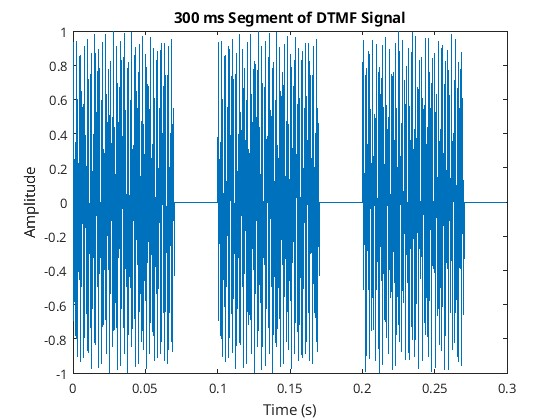
\includegraphics[width=0.5\textwidth]{../Ex04_a.jpg}
   
    It is not easily possible to identify the symbols contained in the segment using just this visualisation since the time domain signal 
    is a superposition of two sinusoidal audio signals with different frequencies

    \item Compute the spectrum for the whole signal and plot its magnitude.
    
      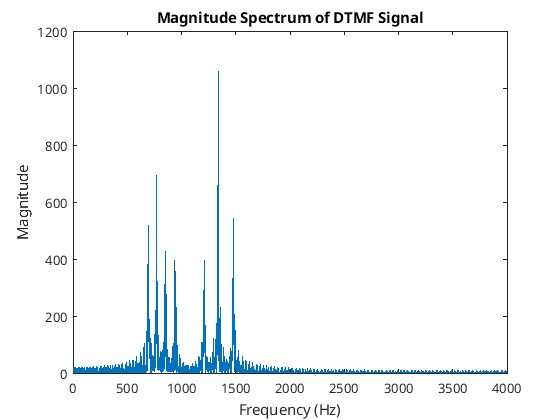
\includegraphics[width=0.5\textwidth]{../Ex04_b.jpg}
   
    \pagebreak

    \item Implement short-time Fourier Transform (STFT). Filter the individual blocks using a Hamming window to improve the spectral
    illustration. Plot a 2d diagram showing the FTBs.

    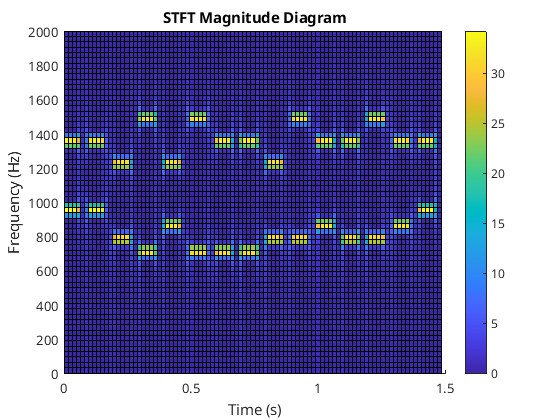
\includegraphics[width=0.5\textwidth]{../Ex04_c.jpg}

    \item Perform the same steps as in (c), but without multiplying the signal blocks by a Hamming window. 
    How does the resulting magnitude diagram of the STFT differ to the one computed in (c)? 
    How is the effect called that causes this difference?

    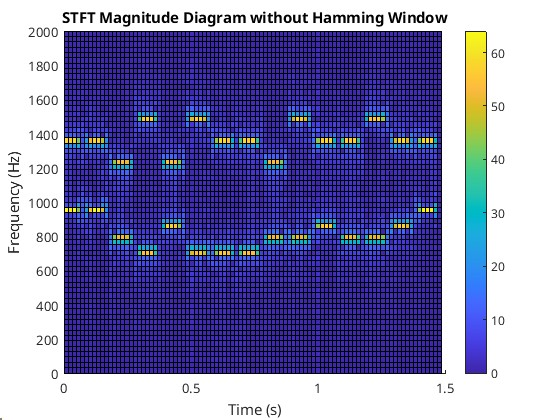
\includegraphics[width=0.5\textwidth]{../Ex04_d.jpg}

    Diagram (c) shows a clearer distinction between frequencies over time, while diagram (d) looks a bit blurry. 
    This is caused by the Hamming windowing process and is done intentionaly to reduces spectral leakage.

    \item On basis of the plotted diagram in (c), determine the symbol sequence that has been used
    for generating the total signal.

    \smallskip

    (0, 0, 4, 3, 7, 3, 2, 2, 4, 6, 8, 5, 6, 8, 0)

    \item
      \begin{enumerate}
        \item What is the essential difference between the diagrams plotted in (b) and (c), and what
        becomes apparent in the diagram in (c) that cannot be observed from the diagram in (b)?

        \smallskip
        (b) shows the frequency spectrum of the entire signal at once, 
        while (c) shows how the frequency content of the signal changes over time. 
        In (c), you can observe the presence of different frequencies at different times, which is not possible in (b).

        \item Give an example for an application of the STFT and describe it briefly.
        
        \smallskip
        Frequencies present in speech signals change rapidly over time.
        STFT allows us to visualize and understand these changes, 
        which can be useful in various applications such as speech signal processing.


      \end{enumerate}
        

  \end{enumerate}

\end{aufgabe} \pagebreak

\begin{aufgabe}{} % Exercise 5 ---------------------------------------------------------
  We have a signal consisting of two cosine oscillations with close frequencies.

  \begin{enumerate}
    \item Compute the (discrete) spectrum of x and plot a line plot of its magnitude.
   
    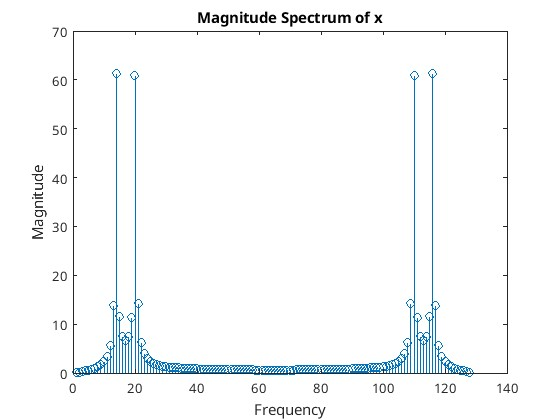
\includegraphics[width=0.5\textwidth]{../Ex05_a.jpg}

    \item Generate and multiply a Hamming window with the signal x to obtain the signal y. Compute the spectrum of y
    and display its magnitude
   
    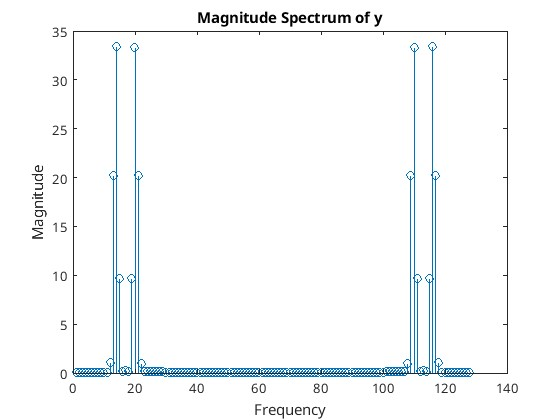
\includegraphics[width=0.5\textwidth]{../Ex05_b.jpg}

    \item Compare and interpret the results from (a) and (b)
    
    They have similar patterns, however the peaks in spectrum y (signal with hamming) are more 
    distinct and less spread out since the hamming window leads to a clearer distinction between the close frequencies.
    
    \item Experiment with w1 and w2 andfind a setting, where the DFT/FFT
    yields the exact result. Explain why the DFT/FFT result is exact with the selected settings.

    The best result is achieved when the sin fits into the signal a whole number of times.
    In this case we need that $w1 * N / (2 * pi)$ and $w2 * N / (2 * pi)$ for some $w1$ and $w2$ will give whole numbers. \\
  \end{enumerate}

\end{aufgabe} \pagebreak

\end{document}
